\newpage
\section{State-of-the-art}

\subsection{Keywords}
Reservoir computing ·  Timeseries · Echo state network · Signal distortion · real-time audio processing · deep reservoir computer · delayed-feedback

\subsection{Core Concepts}

Before exploring many Reservoir computing models and looking for the better suited for our needs, we will first define some core concepts. 

\vspace{0.5cm}

\textbf{General Time Series Processing} refers to the computational analysis of data indexed in chronological order. This includes any signal that evolves over time—such as sinusoids, audio signals, or stock market fluctuations—where each data point at time $t$ is analyzed in relation to its preceding $(t-1)$ and succeeding $(t+1)$ states.

\vspace{0.5cm}

\textbf{Reservoir computing} is a mathematical paradigm belonging to the machine learning field, composed of an input-dependent dynamical system (the reservoir) and a readout trained to compute the desired output from the reservoir state.

\vspace{0.3cm}

This definition is quite hard to produce and maybe not the best since in the literature we often find that reservoir computing is the collectively known mix between ESN and LSM.\cite{holzmann2010echo}.

\vspace{0.3cm}

Some say it is based upon the idea of temporal signal processing on fixed weights.\cite{wyffels2008band}.

\vspace{0.3cm}

In fact, to the best of my knowledge, no official definition was given and reservoir computing is often defined as the ESN\cite{Jaeger10ESN} approach of Jaeger. \cite{Gallicchio2017}. 

\vspace{0.5cm}

\textbf{Nonlinearity} "is a property of mathematical functions or data that cannot be
graphed on straight lines, systems whose output(s) are not directly proportional to
their input(s), objects that do not lie along straight lines, shapes that are not composed of straight lines, or events that are shown or told out-of-sequence." definition from Wikipedia \cite{WikiNonlinearity}.

\vspace{0.5cm}

\textbf{Fading memory} refers to the property of a Reservoir Computing (RC) system to gradually "forget" its initial conditions\cite{Jaeger10ESN}. As the reservoir processes an input stream, the influence of past states decays over time, ensuring that the system's internal dynamics depend primarily on the most recent history of the signal. 

\vspace{0.3cm}

\textbf{Time dependence} Mathematically, the \textbf{hidden state} ($x(t)$) of the reservoir is defined as a function of the entire history of previous timesteps $\{u(t), u(t-1), \dots, u(t - n)\}$ provided to the system \cite{peixeiro2022time}. 

\vspace{0.3cm}

The \textbf{Echo State Property (ESP)} is the fundamental mathematical requirement that bridges these concepts. In essence, the ESP is the combination of a fading memory and the functional dependence of the state on the input: it ensures that hidden states disappear by feeding it in new data, allowing the current dynamics to be driven solely by the continuous input stream.

\vspace{0.5cm}

\subsubsection{Inputs, Time series, signal}

For the purpose of this paper, the terms \textit{input}, \textit{time series}, \textit{signal}, and \textit{sound} are treated as \textbf{interchangeable}. We define these as \textbf{discrete-time} datasets \cite{zolzer2002dafx}, represented as a sequence of observations where each point is indexed by a specific time step.

\begin{figure}[H]
    \centering
    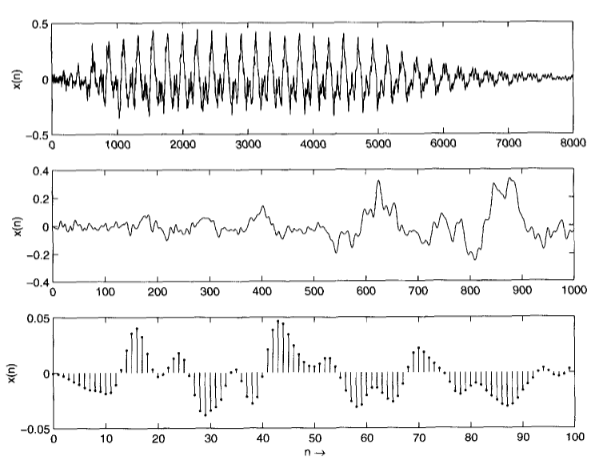
\includegraphics[width=0.75\linewidth]{audio_signal.png}
    \caption{Different time representations for digital audio signals \cite{zolzer2002dafx}}
    \label{fig:audio_signals}
\end{figure}

A standard computer typically processes audio signals at a \textbf{sampling frequency} of \textbf{44.1 kHz} \cite{zolzer2002dafx}, which means we have 44,100 data points (or samples) per second. 

\vspace{0.5cm}

Each sample's amplitude is quantized and stored as a fixed number. For a \textbf{16-bit depth} representation, this corresponds to $2^{16} = 65,536$ possible values, included in [-32,768; 32,767] \cite{zolzer2002dafx}. 
Stereo quality implies that all those measurements are taken twice (one sequence for the left channel and one for the right).

\vspace{0.5cm}

The audio is recorded by an \textbf{ADC (Analog-to-Digital Converter)}, which samples the continuous wave into bits stored inside the computer. It is then processed and sent to a \textbf{DAC (Digital-to-Analog Converter)} to reconstruct an analog signal \cite{zolzer2002dafx} that is as close as possible to the human ear's perception, though never perfectly identical to the original.

\vspace{0.5cm}

Today, ADC and DAC are usually integrated directly into the computer's motherboard.

\vspace{0.5cm}

In order to keep our computation within a delay that the human ear cannot recognize, we must respect the following delays:
\begin{itemize}
    \item \textbf{Less than 15ms}: the human ear doesn't hear a temporal delay \cite{zolzer2002dafx}.
    \item \textbf{Between 10 and 25ms}: perceived as a chorus effect (a form of superposition of the same signal but repeated with echo) \cite{zolzer2002dafx}.
    \item \textbf{More than 50ms}: latency is clearly perceived by the human ear \cite{zolzer2002dafx}.
\end{itemize}

\subsubsection{Benchmarks}

We will also define some of the most widely used benchmarks in the reservoir computing field. 

First, the most common benchmark found in the literature \cite{Jaeger10ESN, holzmann2010echo, wyffels2008band, goldmann2020deep, Gulina17Chaos, Gulina23Koopman} is the \textbf{Mackey-Glass system}. Originally introduced in the field of medical biology, this chaotic time series is named after Michael Mackey and Leon Glass from their seminal 1977 paper \cite{mackey1977oscillation}. The dynamics of the Mackey-Glass is governed by a nonlinear delay differential equation, defined as:
\begin{equation}
    \frac{dy(t)}{dt} = \frac{\alpha y(t-\tau)}{1 + y(t-\tau)^\beta} - \gamma y(t)
\end{equation}
where $y(t)$ is the state variable, $\tau$ is the time delay and $\alpha$, $\beta$, and $\gamma$ are the system parameters.

We must keep in mind that the greater the delay $\tau$, the harder it becomes to predict the next value.

\begin{figure}[H]
    \centering
    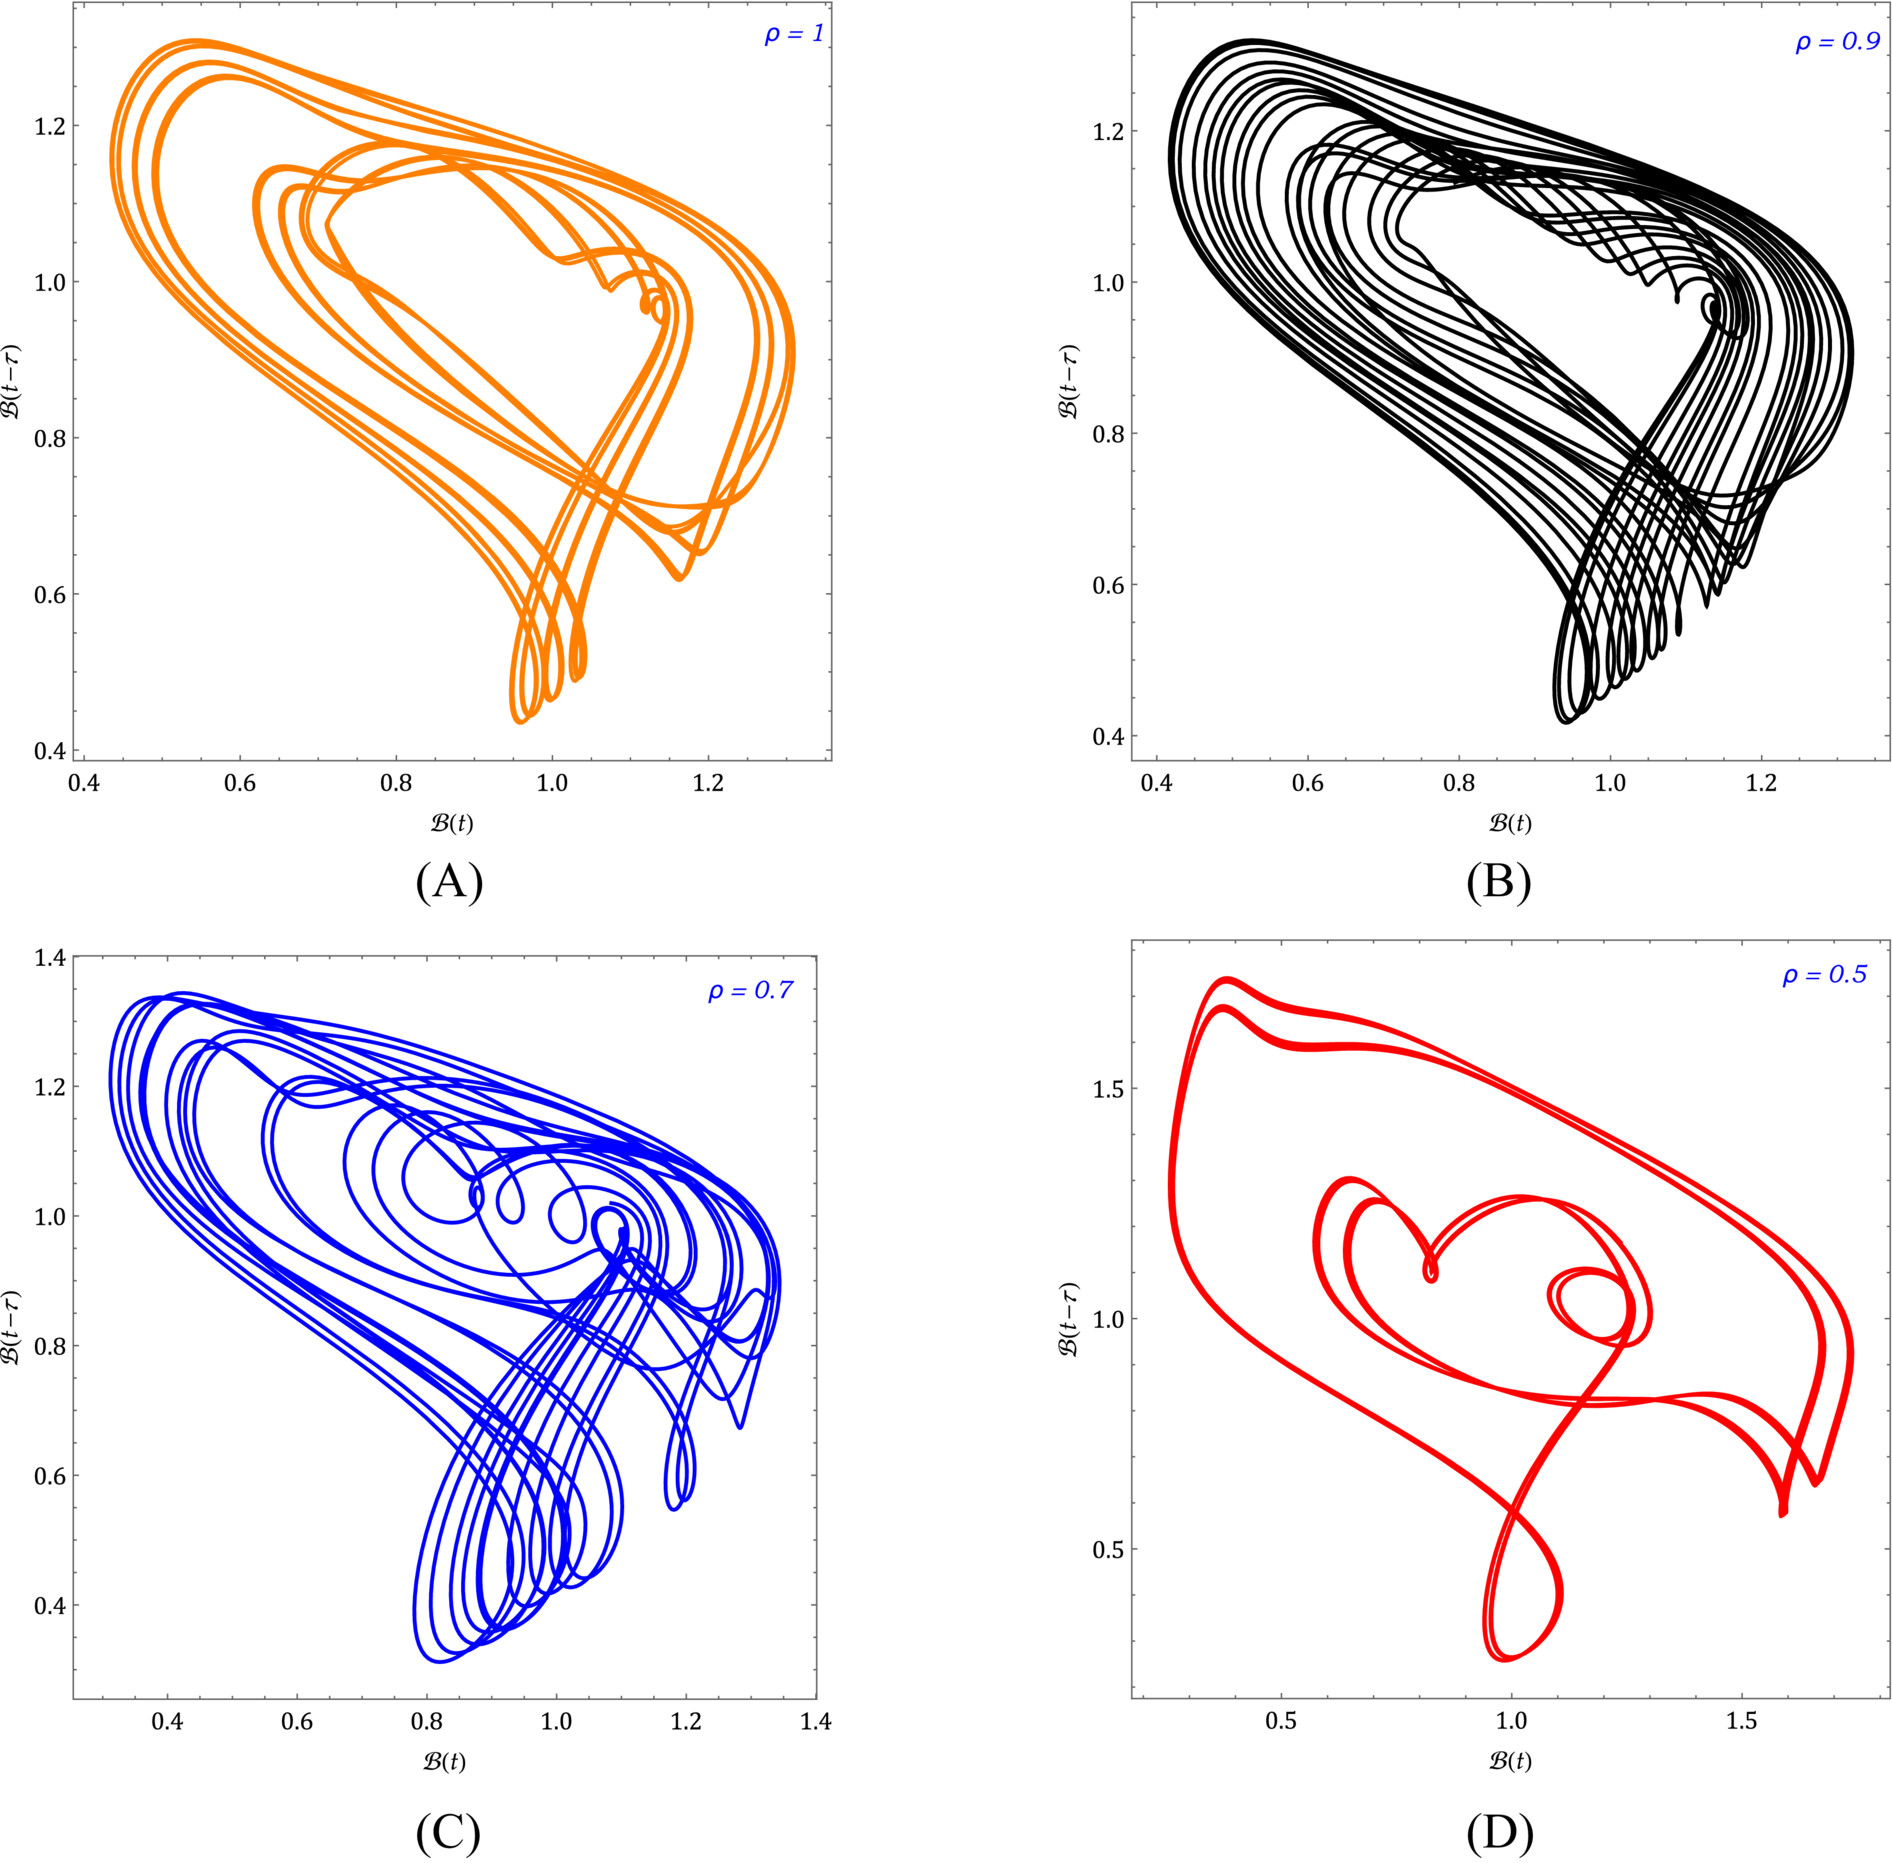
\includegraphics[width=0.75\linewidth]{MG.png}
    \caption{Parametric nature of the system for varying $\rho$ ((A) 1, (B) 0.9, (C) 0.7, and (D) 0.5) combined with $\kappa = 10$, $\tau = 1.5$, $\mu = 1$, and $\alpha = 2$ \cite{wiley_10381}.}
    \label{fig:mackey_glass}
\end{figure}

Even though the Mackey-Glass system does not represent real-time audio distortion, it is still a benchmark used in almost every paper reviewed for this state-of-the-art. In fact, it shares several properties with real-time audio forecasting: it is a \textbf{chaotic, non-linear system}, and it is \textbf{past-dependent}. Because of these similarities, we will use it in this paper as an indicator of a model's ability to compute the desired distortion.

\vspace{0.5cm}

Another widely used benchmark is \textbf{spoken digit recognition} \cite{Appeltant2011Information, schrauwen2008improving}. Although it also relies on audio signals, it is fundamentally a classification task rather than a predictive one, which is why it will not be covered here.

\subsection{Introduction}

We will now look for the best variation of the reservoir computing paradigm for real time audio distortion.
we will study latest and major reservoir computing model and hopefully find the best for real time audio distortion computation. 

\vspace{0.5cm}

Since we will focus on real-time distortion and on standard hardware (consumer laptop without powerful GPU), time complexity $O(n)$ will be focus in our search. 

\subsection{Foundational Models ESN vs LSM}

Several reservoir computing architectures have been proposed, including the Echo State Network (ESN) and the Liquid State Machine (LSM), which share similar core principles but differ in their specific implementations. They are widely recognized in the literature as the foundational models of the \textbf{RC} paradigm.

\subsubsection{The Echo state network}

\vspace{0.5cm}

The Echo State Network (ESN), introduced by Herbert Jaeger \cite{Jaeger10ESN}, belong to the \textbf{RNN} family \cite{jaeger2004harnessing}.\textbf{ESN} relies on the concept that a large, non-linear reservoir can provide the rich dynamics and "echo states" required for signal prediction and modeling. Crucially, these states are mapped to the output by a readout layer that is trained using simple linear regression. This work stands as the foundational paper for ESNs.

\begin{figure}[H] 
    \centering
    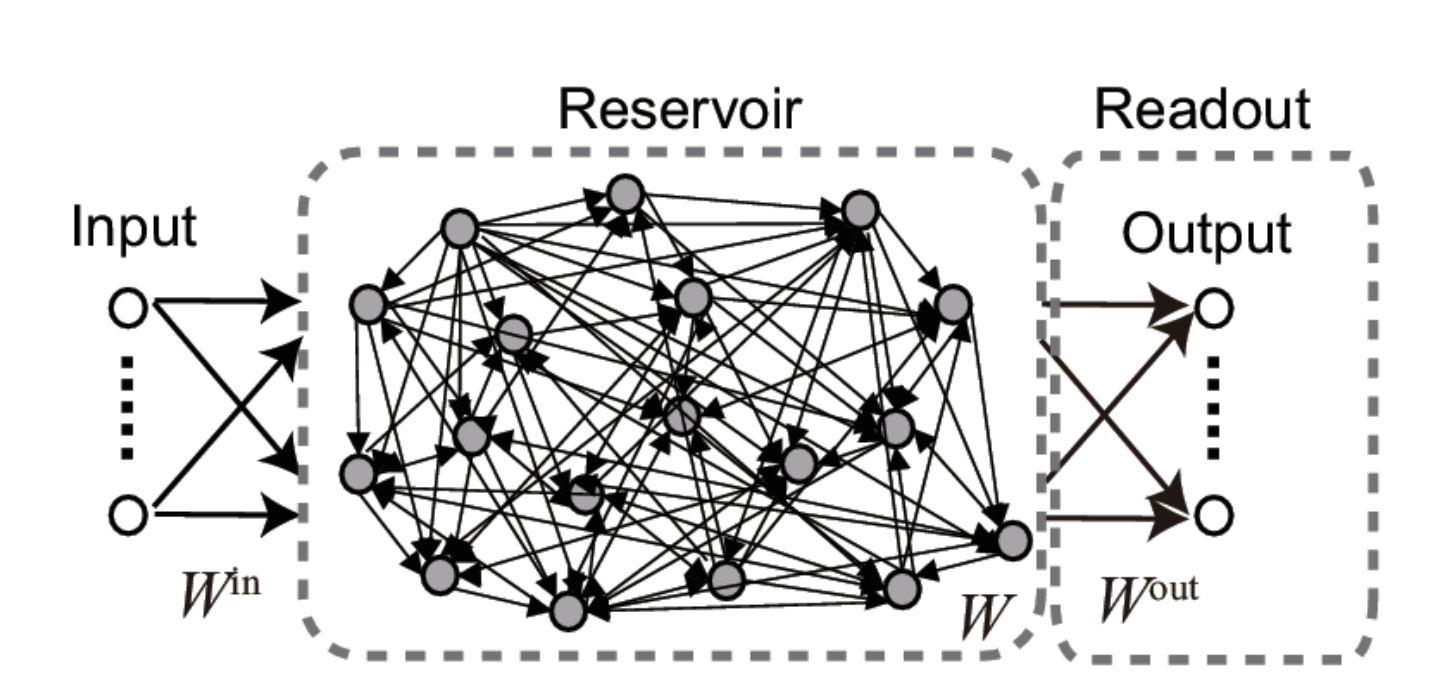
\includegraphics[width=0.75\linewidth]{reservoir_basic.png}
    \caption{Overview of a reservoir computer \cite{VitayNeurocomputing}}
    \label{fig:reservoir}
\end{figure}

As shown in Figure \ref{fig:reservoir}, this architecture is based on three major components:
 \begin{itemize}
     \item \textbf{An input layer:} This feeds the sequential data into the reservoir. Naturally, the time-series data must be ordered chronologically and feed from the oldest to the most recent.
     \item \textbf{A reservoir:} Its primary function is to project the input into state space. Through its fixed recurrent connections and non-linear activation functions, it creates a rich set of dynamics (often referred to as \textbf{interpretable chaos}).
     \item \textbf{A readout layer:} The readout weights are the only trained matrix in this model and generally in the broader Reservoir Computing paradigm, since the internal reservoir connections remain fixed.
 \end{itemize}
 
The idea here is simple: first, we initialize the reservoir's connections using distribution law (with respect over spectral radius) without touching them ever again. Then, we feed the reservoir with an input sequence, and finally, we use linear regression to define the optimal weights for the readout to decode the complex dynamics of the reservoir and get the desired output. "This implies that the training is fast, simple and cannot get stuck in local minima (unlike other training methods)" \cite{holzmann2010echo}.

\textbf{ESN} is characterized by the recurrent feedback loop in their synaptic connection. \cite{jaeger2004harnessing} giving him dynamic memory.

\vspace{0.5cm}

The first hidden state equation given by Jaeger is :
\begin{equation}
    \mathbf{x}(n+1) = f(\mathbf{W}_{in} \mathbf{u}(n+1) + \mathbf{W} \mathbf{x}(n) + \mathbf{W}_{back} \mathbf{y}(n))
\end{equation}
with:
\begin{itemize}
    \item $\mathbf{x}(n)$ is the $N$-dimensional state vector of the reservoir.
    \item $\mathbf{u}(n+1)$ is the external input signal at time $n+1$.
    \item $\mathbf{y}(n)$ is the output signal of the previous step.
    \item $\mathbf{W}_{in}$ is the input weight matrix.
    \item $\mathbf{W}$ is the fixed recurrent weight matrix of the reservoir.
    \item $\mathbf{W}_{back}$ is the optional output feedback weight matrix.
    \item $f$ is the nonlinear activation function of the reservoir nodes, typically the hyperbolic tangent ($\tanh$).
\end{itemize}

\vspace{0.5cm}

Once we compute the internal states $\mathbf{x}(n)$, the optimal readout weights can be computed offline using a standard Ordinary Least Squares (OLS) linear regression:
\begin{equation}
    \mathbf{W}_{out} = (\mathbf{X}^T \mathbf{X})^{-1} \mathbf{X}^T \mathbf{Y}_{target}
\end{equation}

To achieve stability, the reservoir's weight matrix is scaled so that its \textbf{spectral radius} ($\rho(W)$) is maximal (singular or eigen) value, is strictly less than one.

The spectral radius is mandatory to keep the \textbf{ESP}.

The mathematical implications of the spectral radius are explained in more detail by Jaeger \cite{Jaeger10ESN} and Yperman \cite{yperman2016bayesian}.

\vspace{0.5cm}

As always the ESN, as its name implies, and like any other echo model, is the \textbf{Echo State Property (ESP)} defined previously.

\vspace{0.5cm}

Jaeger defines the \textbf{leaky integrator neuron model}, which is used to learn slower dynamical systems (like slow sinusoids). The idea here is to slow down the internal dynamics of the reservoir to stabilize it for slower timescales \cite{Jaeger10ESN}.
Leaky integrator neurons can also maintain the dynamics of a reservoir if the input stops abruptly.
The evolution of a continuous-time leaky integrator network is governed by the following differential equation:
\begin{equation}
    \mathbf{\dot{x}} = C \left( -a\mathbf{x} + f(\mathbf{W}_{in} \mathbf{u} + \mathbf{W} \mathbf{x} + \mathbf{W}_{back} \mathbf{y}) \right)
\end{equation}

where $C$ is a global time constant, $a$ is the leaking decay rate, and $f$ is the nonlinear activation function (typically $\tanh$) \cite{Jaeger10ESN}.

\vspace{0.5cm}

Jaeger pursues optimization and conducts further experiments on leaky-integrator neurons in \cite{jaeger2007optimization} by using a gradient descent loss function over hyperparameters. However, as this paper focuses more on slow dynamics and classification, it has little to no added value for this state of the art.

\vspace{0.5cm}

We can also note that Jaeger provides another, simpler paper regarding ESN implementation, which includes various numerical examples. \cite{jaeger2002tutorial} This paper is intended to be a 'gentle' and 'detailed' guide for the Echo State Network approach. It features practical demonstrations, such as a sinusoid generator, to illustrate the ESN dynamics and training process.

\vspace{0.5cm}

It is also worth noting, standard \textbf{ESN} was successfully used by jaeger in \cite{jaeger2004harnessing} to reduce error-rate signal in cellular communication, emulating the older volterra DFE system in use in that period.

\vspace{0.5cm}

As we will see later in this paper, Even if standard ESNs are an effective paradigm for modeling non-linear distortion, they are computationally demanding. The O(N²) complexity required for the matrix multiplications at each time step makes large ESNs impractical for real-time audio distortion processing on standard hardware (CPU or GPU).

\vspace{0.5cm}

Other limitations of the \textbf{ESN} include difficulties in learning patterns based on multiple timescale signals, as well as a significant \textbf{warm-up} period, defined as the minimal data required to detach the inner state of the reservoir from its initial one.
In our specific case, the short-term memory of the ESN is strictly limited by the size of the reservoir. Since real-time audio processing is computed at higher frequency, all these limitations becomes major. We will discuss the solution proposed by Holzmann and Hauser \cite{holzmann2010echo} later.

\subsubsection{Liquid State Machine (LSM)}

Developed in parallel to Jaeger work on Echo State Networks (ESN) \cite{Jaeger10ESN}, Wolfgang Maass introduced the \textbf{Liquid State Machine (LSM)} \cite{maass2002realtime}. Both models share the same fundamental Reservoir Computing paradigm: they rely on the \textbf{ESP}. In both approaches, the input is fed into a fixed, non-linear dynamical system, and the resulting states are decoded by a readout layer using linear regression \cite{Jaeger10ESN, maass2002realtime}.

\begin{figure} [H]
    \centering
    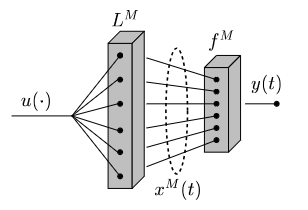
\includegraphics[width=0.6\linewidth]{lsm.png}
    \caption{Liquid state machine \cite{maass2002realtime}}
    \label{fig:lsm}
\end{figure}  

Even if ESNs and LSMs are conceptually identical in their architecture, LSMs typically employ spiking neurons to compute the hidden state, whereas ESNs use discrete-time neurons. 

These spiking neurons get impulses from the previous neurons connected to them, sum them and keep the signal internally, then let the signal fade.

If the neuron gets to a certain maximum point, it discharges itself instantly.

\vspace{0.5cm}

A major distinction that is particularly useful for us lies in the training approach. The standard Jaeger ESN typically uses \textit{offline training}: the entire input sequence is fed into the reservoir to collect all valid states after an initial warm-up (washout) period, followed by a single global linear regression to compute the output weights. Whereas the Maass LSM framework naturally accommodates \textit{online training} \cite{maass2002realtime}. This allows the readout weights to be adjusted iteratively and locally at specific time steps as the system evolves, enabling continuous adaptation to new data without the need to store the entire state history.

\vspace{0.5cm}

Similar to the Echo State Network (ESN) by Jaeger \cite{Jaeger10ESN}, the Liquid State Machine (LSM) suffers from an algorithmic complexity of $\mathcal{O}(N^2)$. This make it unsuitable for real-time audio distortion processing.

\subsection{Enhancing Memory and Multi-Scale Dynamics}

In order to overcome the inherent limitations of foundational models regarding their computational complexity and restricted memory capacity, several architectural upgrades have been proposed. The first modifications we will cover are the integration of Infinite Impulse Response (IIR) filter neurons and the Delay \& Sum readout, which were specifically designed to significantly enhance the short-term memory capacity and manage long-term dependencies \cite{holzmann2010echo}. 

\vspace{0.5cm}

Furthermore, we will introduce the single nonlinear dynamical node with delayed feedback, often referred to as Delay-Line Reservoir Computing. This approach represents a major architectural breakthrough, as it successfully reduces the algorithmic time complexity per sample from $\mathcal{O}(N^2)$ to $\mathcal{O}(N)$ \cite{Appeltant2011Information}.


\subsubsection{Echo state networks with filter neurons and a "delay \& sum" readout}

In 2010, Holzmann and Hauser \cite{holzmann2010echo} improved Jaeger original ESN architecture \cite{Jaeger10ESN} by extending the filter neurons proposed by Wyffels et al. \cite{wyffels2008band} to arbitrary Infinite Impulse Response (IIR) filters,\cite{holzmann2010echo} and by introducing a new delayed readout mechanism. These modifications are particularly suited for complex tasks like real-time audio distortion.

\vspace{0.5cm}

This approach was purposely designed to overcome the short-term memory limitations associated with reservoir size when learning from the distant past. Furthermore, it addresses the strong coupling between neurons that makes it almost impossible for standard ESNs to learn signals composed of multiple attractors or frequencies \cite{holzmann2010echo, Keuninckx2017RealTime}.

\vspace{0.5cm}

They introduced two major improvements over the original ESN: 

\vspace{0.5cm}

First, they integrated arbitrary \textbf{IIR (Infinite Impulse Response)} filters directly into the reservoir neurons.

\begin{figure} [H]
    \centering 
    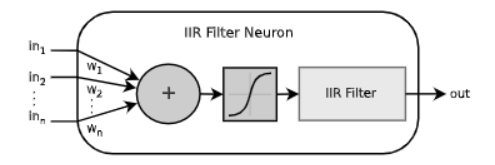
\includegraphics[width=0.6\linewidth]{IIR.png} 
    \caption{IIR Filter neuron \cite{holzmann2010echo}} 
    \label{fig:iir_filter} 
\end{figure}

The main objective of these \textbf{IIR} filters is to specialize neurons to different frequency bands, enabling the ESN to successfully model multiple attractors.

\vspace{0.5cm}

This filter is placed immediately after the nonlinear activation of every reservoir cell. Consequently, the system performs a two-step computation. First, the standard reservoir update determines an intermediate state $\tilde{x}_i(n+1)$. 
\begin{equation}
    \tilde{x}_i(n+1) = f \left( \rho \mathbf{W}_i \mathbf{x}(n) + \mathbf{W}_{in,i} \mathbf{u}(n+1) + \mathbf{W}_{fb,i} \mathbf{y}(n) + \upsilon(n+1) \right)
\end{equation}
where $\mathbf{W}_i$, $\mathbf{W}_{in,i}$, and $\mathbf{W}_{fb,i}$ represent the $i$-th rows of the respective weight matrices, $\rho$ is the spectral radius, and $f$ is the nonlinear activation function.

Subsequently, the IIR filter is applied to this intermediate value to produce the final state of the cell, $x_i(n+1)$.\cite{holzmann2010echo}:

\begin{equation}
    x_i(n+1) = \frac{1}{a_{i,0}} \left( \sum_{j=0}^K b_{i,j} \tilde{x}_i(n-j) - \sum_{j=1}^K a_{i,j} x_i(n-j) \right)
\end{equation}
where:
\begin{itemize}
    \item $b_{i,j}$ are the fixed weights of the feedforward path to neuron $i$.
    \item $a_{i,j}$ are the fixed weights of the feedback path t neuron $i$.
    \item $K$ determines the order of the digital filter. (how deep neuron keep information)
\end{itemize}

\vspace{0.5cm}

To maintain the \textbf{Echo State Property (ESP)} in this extended architecture, specific stability conditions must be met: as always the spectral radius $\rho$ of the internal weight matrix must remain within $0\leq\rho<1$, \textbf{and} the maximum gain of each individual IIR filter must not exceed 1 \cite{holzmann2010echo}.

\vspace{0.5cm}

Because the parameters for these filters are fixed in advance and specific to each neuron, they do not require additional training, thus preserving the computational efficiency of standard ESNs \cite{holzmann2010echo}.

\vspace{0.5cm}

Secondly, they added a \textbf{delay\&sum (D\&S) readout}.

\begin{figure} [H]
    \centering
    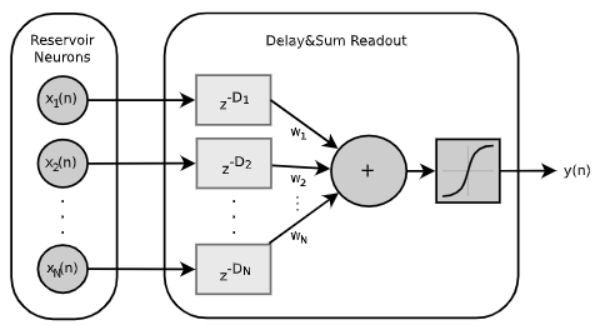
\includegraphics[width=0.8\linewidth]{delayandsum.png}
    \caption{Delay\&Sum readout \cite{holzmann2010echo}}
    \label{fig:delay_sum}
\end{figure}

This \textbf{D\&S readout} is a major upgrade to the ESN, designed to drastically increase the memory capacity of the network. Until now, the memory of the reservoir was strictly limited by its size (the number of neurons) \cite{Jaeger10ESN}. The delay\&sum mechanism computes the optimal temporal delay needed for each synaptic connection to the output, minimizing the loss and allowing the network to retain past information much longer than a traditional reservoir.

\vspace{0.5cm}

Assuming an ESN with $N$ internal units and $L$ inputs, the reservoir and input signals are combined into a single vector $\mathbf{s}(n) = (x_1(n), \dots, x_N(n), u_1(n), \dots, u_L(n))^T$. The $m$-th output $y_m(n)$ of the D\&S readout is computed as:
\begin{equation}
    y_m(n) = g \left( \sum_{i=1}^{N+L} W^{out}_{i,m} s_i(n - D_{i,m}) \right)
\end{equation}
where:
\begin{itemize}
    \item $D_{i,m}$ is the integer delay applied to the signal $s_i$ before reaching the $m$-th output.
    \item $W^{out}_{i,m}$ is the trainable output weight.
    \item $g$ is the activation function of the output neuron.
\end{itemize}

In addition to training the standard readout weights, the delay\&sum readout requires training to find the optimal temporal delay for each connection.

A method proposed by the authors is to estimate the cross-correlation $\hat{r}$ between each internal signal $s_j(n)$ and the target output $t_m(n)$:
\begin{equation}
    \hat{r}_{s_j t_m}(\tau) = \frac{1}{n_{max}} \sum_{n=0}^{n_{max}-1} s_j(n) g^{-1}(t_m(n+\tau))
\end{equation}
where $n_{max}$ is all the information. The optimal delay $D_{j,m}$ for each connection is then chosen as the time shift $\tau$ that maximizes the absolute correlation:
\begin{equation}
    D_{j,m} = \text{arg}\max_{\tau} |\hat{r}_{s_j t_m}(\tau)|
\end{equation}
Once all delays are estimated and fixed, the reservoir and input signals are shifted in time accordingly. The output weights $W^{out}$ are then optimized using a standard offline linear regression on these correctly delayed signals \cite{holzmann2010echo}.

\vspace{0.5cm}

Holzmann and Hauser proposed two different algorithms for training the \textbf{D\&S} readout to find the optimal delay for each neuron, which will require further investigation.

\vspace{0.5cm}

These modifications to the original \textbf{ESN} make this model a strong competitor for real-time audio distortion processing.
Although this architecture is a major upgrade in the \textbf{RC} paradigm, some limitations remain for our objective. First, the computational complexity is still $\mathcal{O}(N^2)$, and as the authors themselves stated, if we try to learn a single attractor instead of multiple ones, the \textbf{IIR} filters perform worse \cite{holzmann2010echo}.


\subsubsection{Delay-line and single dynamical node}

In 2011, Appeltant et al. \cite{Appeltant2011Information} introduced a major architectural improvement to the Reservoir Computing paradigm. Their main objective was to drastically reduce the computational complexity of traditional Echo State Networks. To achieve this, they proposed replacing the large pool of physically interconnected neurons with a single nonlinear node subjected to a delayed feedback loop.

\begin{figure}[H]
    \centering
    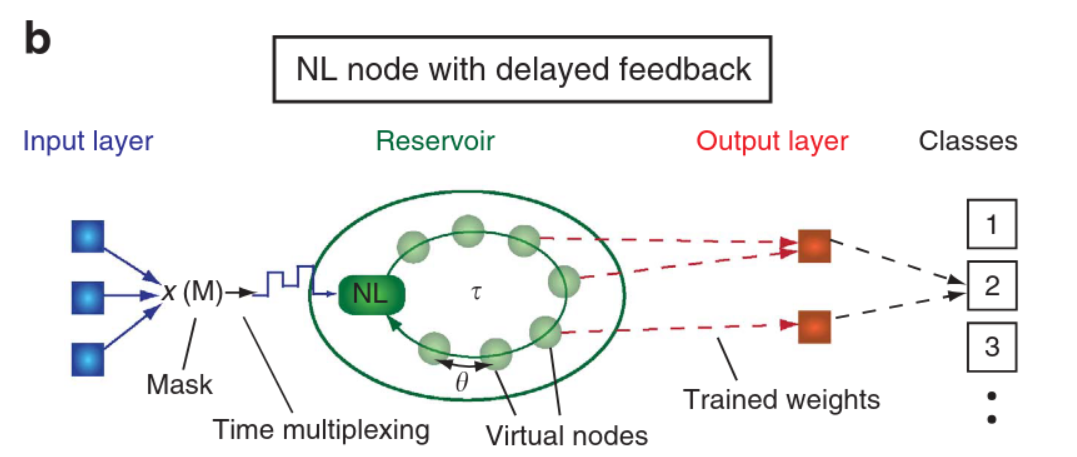
\includegraphics[width=0.75\linewidth]{dlrc.png}
    \caption{Single nonlinear node with delayed feedback \cite{Appeltant2011Information}}
    \label{fig:dlrc_architecture}
\end{figure}

In the \textbf{DLRC} (or Single Node) approach, the node receives its own previous output after a delay time $\tau$. 

It rely on 3 major steps, First \textbf{the masking}: 
Where the discrete-time input sequence $u(n)$ feed the reservoir during full delay period $\tau$. It is then multiplied by a periodic masking signal $M(t)$ consisting of $N$ constant values. The resulting continuous-time masked input $J(t)$ fed into the node \cite{Appeltant2011Information}:
\begin{equation}
    J(t) = M(t) u(n) \quad \text{for } t \in [n\tau, (n+1)\tau]
\end{equation}
where the mask $M(t)$ changes value at fixed intervals $\theta = \tau / N$.

Then the \textbf{masked signal is injected} into the nonlinear node. The update rule for the node state $x(n)$ at discrete time $n$ using Infinite Impulse Response (IIR) \cite{wyffels2008band}:
\begin{equation}
    x(n) = a x(n-1) + (1-a) f \big( \gamma J(n) + \eta x(n-N) \big)
\end{equation}
where:
\begin{itemize}
    \item $x(n)$ is the current state of the system.
    \item $x(n-N)$ is the delayed feedback state from the previous cycle.
    \item $a \in ]0, 1[$ is the filter factor controlling the inertia of the node and the mixing of adjacent virtual states.
    \item $\gamma$ is the input strength.
    \item $\eta$ is the feedback strength.
    \item $f$ is the nonlinear activation function.
\end{itemize}

And finally the linear regression take place like define by Jaeger\cite{Jaeger10ESN}.

To achieve optimal performance, several crucial parameters governing the dynamics of this temporal reservoir must be carefully tuned:
\begin{itemize}
    \item \textbf{Feedback strength} ($\eta$): Controls the influence of the past delayed state on hidden state. It serves a role analogous to the spectral radius in a traditional RC, maintaining the system at the edge of stability.
    \item \textbf{Input gain} ($\gamma$): Determines how strongly the nonlinear node is driven by the external input signal, which is analogous to the input scaling in an ESN.
    \item \textbf{Delay time} ($\tau$): The total duration of the feedback loop. It is directly related to the total number of virtual nodes in the system.
    \item \textbf{Node separation} ($\theta$): The constant time interval between two consecutive virtual nodes in the delay line ($\theta = \tau/N$). Its value determines the mixing of adjacent states, acting similarly to the sparsity of the interconnection matrix in a standard reservoir.
\end{itemize}

This temporal multiplexing approach allows the system to process time-series data efficiently while significantly reducing the computational cost. By replacing heavy matrix multiplications of a standard ESN with a simple time-delay loop, the computational complexity drops from $\mathcal{O}(N^2)$ to $\mathcal{O}(N)$ \cite{Keuninckx2017RealTime} per time step. As discussed later in this paper, a specific discrete-time modification of this paradigm was successfully implemented by Keuninckx et al. \cite{Keuninckx2017RealTime} to model real-time audio distortion.

\subsection{Stacked and Deep Models}

In this section, we will define models under the (RC) paradigm that are composed of multiple reservoirs or layered architectures, such as Delay-Line Reservoir Computing (DLRC) \cite{Appeltant2011Information}, Cascaded DLRC \cite{Keuninckx2017RealTime}, and Deep Time-Delay Reservoir Computing (DeepTRC) \cite{goldmann2020deep}. 

These advanced models emerge as the most suitable candidates to address our research questions. The core principle behind these architectures is to overcome the final computational barriers between the RC paradigm and strict real-time audio processing constraints by:

\begin{itemize}
    \item \textbf{Proposing a hierarchy of timescales:} Layered architectures inherently develop a multiple time-scale organization, allowing the network to naturally capture both short- and long-term temporal dependencies across different levels of abstraction \cite{Gallicchio2017}.
    \item \textbf{Enhancing dynamical richness:} Stacking reservoir layers significantly amplifies the richness of the state dynamics,  increasesing memory capacity without the need for wider, fully connected networks \cite{Gallicchio2017, goldmann2020deep}.
    \item \textbf{Reducing algorithmic time complexity:} By utilizing single nonlinear nodes with delayed feedback and unidirectional coupling, these architectures drastically reduce the computational cost. This design provides a constant, low computation time even as the total number of virtual nodes increases, effectively bypassing previous bottlenecks and making real-time processing achievable on standard hardware \cite{Appeltant2011Information, Keuninckx2017RealTime, goldmann2020deep}.
\end{itemize}


\subsubsection{Deep reservoir computing}

In 2017, Gallicchio et al. \cite{Gallicchio2017} explored the concept of Deep Reservoir Computing, bridging deep learning architectures with the reservoir computing paradigm.

\vspace{0.5cm}

Their idea was to stack multiple reservoirs one on top of the other:

\begin{figure} [H]
    \centering
    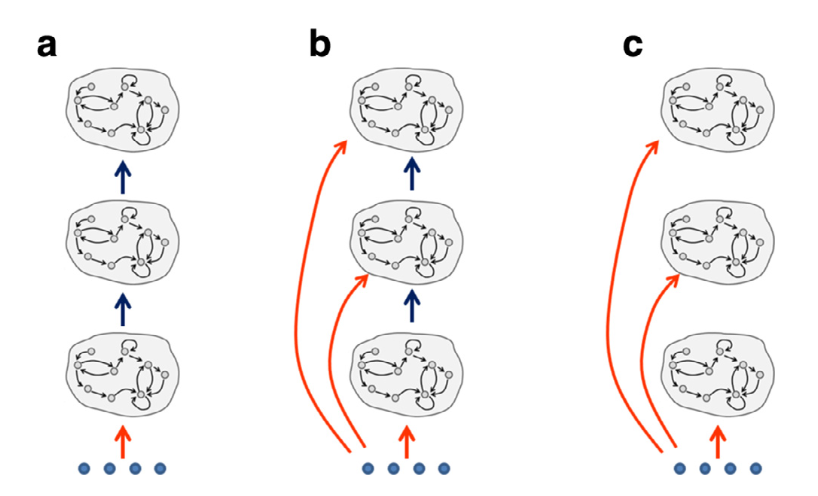
\includegraphics[width=1\linewidth]{deep_esn.png}
    \caption{Deep RC architectures \cite{Gallicchio2017}}
    \label{fig:deep_rc}
\end{figure}

For this purpose, they developed three distinct models based on the ESN paradigm but incorporating deep layers:
\begin{itemize}
    \item \textbf{DeepESN}: (a) The simplest deep architecture, where each reservoir layer directly feeds into the next one.
    \item \textbf{DeepESN-IA} (b) (Input to All): Every layer in the stack receives the external input signal directly.
    \item \textbf{GroupedESN}: (c) Each sub-reservoir receives the external input directly without feeding into the others (they are arranged in parallel rather than stacked).
\end{itemize}

The experiments conducted on these new models revealed that the DeepESN architecture is better suited than a standard ESN processing complex temporal data. It develops hierarchical memory, capturing rapid dynamics (short-term memory) in the first layer and progressively slower dynamics (long-term memory) in the deeper layers. This multiple time-scale representation is highly relevant for our research on real-time audio distortion, as such complex audio signals inherently require modeling both shorter and longer temporal dependencies simultaneously.

\vspace{0.5cm}

Since the benchmarks in \cite{Gallicchio2017} indicate that DeepESN is the only architecture possessing added value for our specific application (short and long term memory), and because the DeepESN-IA and GroupedESN models were primarily introduced as baselines to isolate the effects of layering, these two models will not be explored further in this study.

\vspace{0.5cm}

First, the first reservoir is fed using the external input sequence and each successive layer is fed directly by the output state of the previous one. The input $\mathbf{i}^{(l)}(t)$ for the $l$-th layer at time step $t$ is thus defined as \cite{Gallicchio2017}:
\begin{equation}
    \mathbf{i}^{(l)}(t) = 
    \begin{cases} 
        \mathbf{u}(t) & \text{if } l = 1 \\
        \mathbf{x}^{(l-1)}(t) & \text{if } l > 1 
    \end{cases}
\end{equation}

the internal state $\mathbf{x}^{(l)}(t)$ of each layer $l$ is updated at each discrete time step $t$ according to the following state transition function \cite{Gallicchio2017}:
\begin{equation}
    \mathbf{x}^{(l)}(t) = (1 - a^{(l)}) \mathbf{x}^{(l)}(t - 1) + a^{(l)} \tanh \left( \mathbf{W}_{in}^{(l)} \mathbf{i}^{(l)}(t) + \mathbf{\hat{W}}^{(l)} \mathbf{x}^{(l)}(t - 1) + \boldsymbol{\theta}^{(l)} \right)
\end{equation}
where:
\begin{itemize}
    \item $a^{(l)} \in [3]$ is the leaky parameter for layer $l$, controlling the speed of its dynamics.
    \item $\mathbf{W}_{in}^{(l)}$ is the initialized input weight matrix for layer $l$.
    \item $\mathbf{\hat{W}}^{(l)}$ is the recurrent weight matrix of layer $l$.
    \item $\boldsymbol{\theta}^{(l)}$ is the bias-to-reservoir weight vector for layer $l$.
\end{itemize}

Then the output weight are computed using a linear regression, the author also mention de Ridge regression to prevent overfitting.

To compute the final output, once training is complete, The network's output $\mathbf{y}(t)$ is computed as a linear combination of all layers \cite{Gallicchio2017}:
\begin{equation}
    \mathbf{y}(t) = \mathbf{W}_{out} [\mathbf{x}^{(1)}(t), \mathbf{x}^{(2)}(t), \dots, \mathbf{x}^{(N_L)}(t)]^T + \boldsymbol{\theta}_{out}
\end{equation}
where $\mathbf{W}_{out}$ is the readout weight matrix and $\boldsymbol{\theta}_{out}$ is the bias-to-readout vector \cite{Gallicchio2017}.


\vspace{0.5cm}

The other experiments discussed in \cite{Gallicchio2017} involve the use of \textbf{Intrinsic Plasticity (IP)}, sometimes referred to as homeostatic plasticity. This concept was formally adapted to the RC paradigm by Schrauwen et al. \cite{schrauwen2008improving}, extending the foundational work of Triesch \cite{triesch2005gradient}.

\vspace{0.5cm}

To be completely honest, understanding the IP in detail requires a deep understanding of biology and mathematics that goes way beyond me. From what I understand, essentially, IP is a local, learning rule that allows each individual neuron to fine-tune the gain and bias of its own activation function. By forcing the neuron's output to follow a target probability distribution, the rule maximizes the entropy within the reservoir. This ensures the neurons do not saturate.

As summarized by the authors:
\begin{quote}
"The simple, local IP rule effectively makes reservoirs significantly more robust: it empowers the reservoirs with the ability to autonomously and robustly adapt their internal dynamics, irrespective of initial weight setting, input scaling or topology, to a dynamic regime which is suited for the given task. The rule is purely input driven, and adapts the reservoir in an unsupervised way." \cite{schrauwen2008improving}.
\end{quote}


\subsubsection{Cascade of Discrete-Time Delay Line-Based (DLRC)}

In 2017, Keuninckx, Danckaert, and Van der Sande \cite{Keuninckx2017RealTime} revisited the single dynamical node concept originally defined by Appeltant et al. (2011) \cite{Appeltant2011Information} and expanded upon it by integrating the IIR filter neuron approach proposed by Holzmann \cite{holzmann2010echo}. While the standard DLRC was effective for simpler tasks, although identified significant limitations when applied to the complex dynamics of a guitar amplifier. This specific task requires both a long memory (for the acoustic response) and a strong nonlinearity ,requirements that a standard ESN or a single-node DLRC could not solve alone.

\begin{figure} [H]
    \centering
    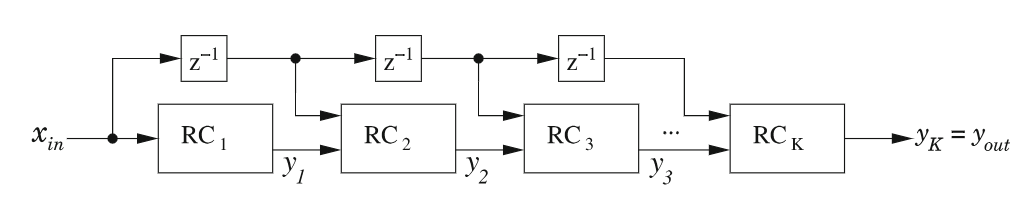
\includegraphics[width=0.75\linewidth]{casc.png}
    \caption{Cascade of discrete-time delay line reservoir computer \cite{Keuninckx2017RealTime}}
    \label{fig:cascade_dlrc}
\end{figure}

To overcome this, Keuninckx proposed a novel architecture: a cascade of $k$ reservoirs, each containing 100 virtual nodes\cite{Appeltant2011Information}. The 'genius' of this approach lies in its multiplexing strategy, passing both the original guitar signal $x_{in}$ and the previous layer output $y_{i-1}$ to the next reservoir.
The use of filtered virtual neurons \cite{Appeltant2011Information} to match audio timescales. This structure successfully emulated the rich sound of guitar amplifier in real-time on standard hardware (a consumer laptop), demonstrating the ability of reservoir computer paradigm for nonlinear audio signal real-time distortion at 44.1 kHz.

\vspace{0.5cm}

To process the audio signal effectively, their discrete-time architecture relies on the use of an \textbf{input mask} \cite{Appeltant2011Information, Keuninckx2017RealTime}. The mask is defined as a periodic sequence of size $N$, where $N$ is the number of virtual nodes composing the feedback loop. At each time interval, the incoming audio sample is multiplied by the mask values. This crucial step distributes the signal across the virtual nodes, maintains the entropy inside the reservoir, and keeps the dynamics in a "transient state"\cite{Keuninckx2017RealTime}, preventing the system from relaxing into a stable equilibrium.

\vspace{0.5cm}

\begin{figure}[H]
    \centering
    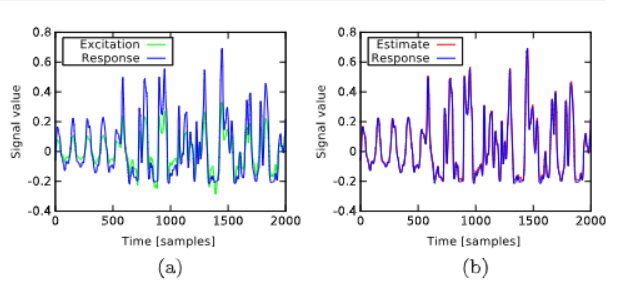
\includegraphics[width=1\linewidth]{comparaison_cascade.png}
    \caption{comparison of single vs cascade delayed feedback} \cite{Appeltant2011Information}
    \label{fig:comparaison_cascade}
\end{figure}

The results displayed in the upper graph illustrate a precision comparison between the \textbf{Cascaded delayed feedback} architecture \cite{Keuninckx2017RealTime} and the standard \textbf{DLRC} \cite{Appeltant2011Information}. They demonstrate a clear superiority of the cascaded architecture, showing a near-perfect match between the expected and obtained results. 

\vspace{0.5cm}

To the best of our knowledge, Keuninckx and his team are the only researchers to have conducted real-time audio distortion tests at 44.1 kHz with such low latency. Although they did not explicitly state a global latency time in milliseconds, their architecture introduces an algorithmic delay of exactly one sample per reservoir unit \cite{Keuninckx2017RealTime}. For a 5-unit cascade at 44.1 kHz, this corresponds to a delay of merely 5 samples (approximately 0.11 ms), which is far below the 15 ms previously defined. 

\vspace{0.5cm}

This exceptional real-time performance and precision make this architecture a clear choice for further testing on other real-time audio distortion tasks.

\vspace{0.5cm}

At this point, our reading confirmed that some models under the Reservoir Computing paradigm is viable for real-time audio distortion, but the relevant paper being somewhat dated (2017). Therefore, the remainder of this state of the art focuses on the newest optimizations of the paradigm, such as the Next Generation Reservoir Computer \cite{Gauthier2021} and Deep Time-delay reservoir computer. We cover in the next chapter to determine if these new models can achieve better results than the methods previously established.

The work produced by Gallicchio et al. \cite{Gallicchio2017} represents a significant step forward in our search for a model under the \textbf{RC} paradigm capable of real-time audio processing. The DeepESN architecture defined there, with its ability to simultaneously capture both short and long memory patterns, will be precious in this regard.


\subsubsection{Deep Time-Delay Reservoir Computer (deepTRC)}

In 2020, Mirko Goldmann and his team introduced a new model \cite{goldmann2020deep} based on the foundational works of Jaeger \cite{Jaeger10ESN}, Appeltant \cite{Appeltant2011Information}, and Gallicchio \cite{Gallicchio2017}.

This new \textbf{deepTRC} architecture is a hybrid approach that merges \textbf{Deep Reservoir Computing} \cite{Gallicchio2017} with the \textbf{DLRC}) paradigm \cite{Appeltant2011Information}. 

\begin{figure} [H]
    \centering
    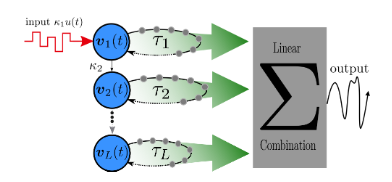
\includegraphics[width=0.65\linewidth]{deep_time_delay.png}
    \caption{Deep time-delay reservoir computer \cite{goldmann2020deep}}
    \label{fig:deep_trc}
\end{figure}

In this architecture, the external input signal is fed exclusively to the first layer. This initial layer processes the input signal using the nonlinear delay node model proposed by Appeltant \cite{Appeltant2011Information}.

\vspace{0.5cm}

This unidirectional process continues sequentially for every layer in the model.

\vspace{0.5cm}

Once the continuous state of a layer is computed, it is multiplied by a coupling gain and is instantaneously used to feed the next layer. It is worth noting that while the external input gain applied to the first layer is often greater than one, the inter-layer coupling gains are typically smaller, acting as linear filters.

\vspace{0.5cm}

Once the initial warm-up (washout) period is completed and the entire input sequence has been fed, the states from all virtual nodes across all layers are extracted. These combined states are then used simultaneously to train the readout weights with single global linear regression.

\vspace{0.5cm}

Even if this model was not directly tested on real-time audio distortion processing, this architecture has strong similarities with other models previously studied and is reduce warm-up phase\cite{Gulina17Chaos}.

\vspace{0.5cm}

Consequently, the Deep Time-Delay Reservoir Computing \textbf{(deepTRC)} architecture emerges as a highly promising candidate for subsequent testing phases. By leveraging a layered topology, it inherently benefits enhanced short-term memory capacity and greater richness of state dynamics, sharing fundamental properties with previous models \cite{Keuninckx2017RealTime, Gallicchio2017, Appeltant2011Information}. 

\vspace{0.5cm}

Furthermore, because its architecture closely resembles the cascaded DLRC approach \cite{Keuninckx2017RealTime}, the deepTRC is expected to achieve comparable real-time processing capabilities without prohibitive computational overhead. Indeed, its algorithmic time complexity scales linearly with the total number of virtual nodes ($L$ layers $\times N$ nodes per layer), strictly bypassing the $\mathcal{O}(N^2)$ bottleneck of classical \textbf{ESN}. Combined with its proven high predictive accuracy on chaotic benchmarks \cite{goldmann2020deep}, this optimal trade-off between dynamical richness and computational efficiency makes it a particularly strong model to address our specific research questions.

\subsection{Emerging Paradigms and Recent Advancements}

This final section reviews the most recent advancements in the literature, specifically the Next Generation Reservoir Computing (NG-RC) \cite{Gauthier2021} and the Volterra kernel \cite{gonon2025reservoir}.

These latest models under the \textbf{RC} paradigm will be examined to evaluate their potential to overcome the limitations of previously discussed architectures. Any significant improvements over earlier models will be assessed, with a particular focus on reductions in algorithmic time complexity, enhancements in memory capacity, and increased predictive precision.

\subsubsection{Next Generation Reservoir Computing (NG-RC)}

The \textbf{Next Generation Reservoir Computing (NG-RC)}, which is mathematically identical to Nonlinear Vector Autoregression (NVAR), has been proven to be equivalent to a linear RC \cite{Gauthier2021}. It excels at standard benchmark tasks while offering similar or better performance compared to traditional ESN.

The core concept here is to eliminate the reservoir. Instead of broadcasting the input into  reservoir, the NG-RC creates a feature vector directly from time-delayed observations of the input data and their nonlinear functionals \cite{Gauthier2021}. The output weight matrix is then applied directly to these features.

\begin{figure}[H]
    \centering
    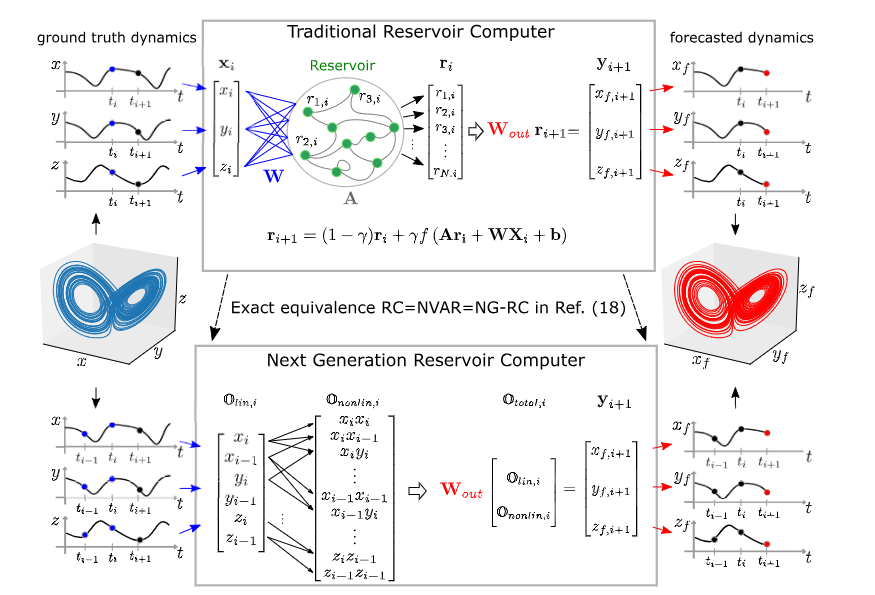
\includegraphics[width=0.95\linewidth]{NGRC.png}
    \caption{Exact equivalence between a traditional RC and the NG-RC architecture \cite{Gauthier2021}}
    \label{fig:ng_rc}
\end{figure}

According to the authors, \textbf{the NG-RC requires a dramatically shorter warm-up period} \cite{Gauthier2021}. This property has two significant impacts. First, it \textbf{decreases required length of datasets}, since very few data points are discarded during the warm-up phase \cite{Gauthier2021}. Second, in our specific case of real-time audio transformation, this minimal warm-up requirement can \textbf{drastically speed up the initialization} of the system, making it a good candidate for testing real-time processing applications.

\vspace{0.5cm}

Note that although \textbf{NG-RC} is presented in the literature as mathematically equivalent to \textbf{ESN} \cite{Gauthier2021}, offering reduced computational complexity $\mathcal{O}(n)$, it is unlikely strong enough (in his architecture) to capture the rich dynamics we are looking for here. Indeed, it has not yet been compared to more capable models in our field. Currently, the only models known in the literature capable of handling such complex tasks rely on layered architectures, which provide greater richness in their memory and state dynamics for subsequent decoding \cite{goldmann2020deep, Keuninckx2017RealTime}.

\subsubsection{The Volterra Kernel}

Finally in 2025 Grigorveya at al. \cite{gonon2025reservoir}.
Based on the theory of Reproducing Kernel Hilbert Spaces (RKHS), a complex mathematical vector family and the Volterra series representation, built a new framework within the reservoir computing family \cite{gonon2025reservoir}. This model possesses the following properties:
\begin{itemize}
    \item It can approximate any causal and time-invariant filter with the fading memory property \cite{gonon2025reservoir}.
    \item It is efficiently computable via explicit recursions \cite{gonon2025reservoir}.
    \item It is sequentially updatable, making it suitable for computing time series \cite{gonon2025reservoir}.
    \item It is a universal kernel, meaning it can approximate any nonlinear system with \textbf{ESP} \cite{gonon2025reservoir}.
\end{itemize}

This new paradigm is built upon the \textbf{Volterra reservoir kernel}. However, understanding the Volterra series and RKHS requires an advanced mathematical background and a dedicated state-of-the-art review. Furthermore, this approach is likely overkill for real-time audio distortion processing. 

\vspace{0.5cm}

Finally, based on our understanding of its presentation \cite{grigoryeva_video}, the computation of such a model requires a third-order tensor and a regression performed in an infinite-dimensional space. Therefore, we can reasonably assume that the computation of a single time step with a complexity of $\mathcal{O}(n^3)$. As previously noted in the literature regarding Volterra series \cite{Keuninckx2017RealTime}, this increase in computational complexity severely limits their real-time applicability for audio processing at a 44.1 kHz sampling rate. 

\subsection{Bayesian Optimization of Hyper-parameters}

Although it does not introduce a new Reservoir Computing model strictly speaking, the work of Yperman and Becker \cite{yperman2016bayesian} is highly relevant to our search for the optimal architecture for real-time audio processing.

\vspace{0.5cm}

Their study describes an automated search method using a Gaussian process combined with Bayesian optimization to find the best hyperparameters of a reservoir \cite{yperman2016bayesian}. This technique allows efficient and simultaneous optimization of multiple variables such as spectral radius, input scaling, number of neurons, and regularization parameter.

\vspace{0.5cm}

This approach has proven to be a powerful alternative to manual or random search strategies. By intelligently navigating the error surface to balance the exploitation of known good regions with the exploration of uncertain ones, Bayesian optimization significantly reduces the need for expert and converges toward an optimal set of hyperparameters \cite{yperman2016bayesian}.

\vspace{0.5cm}

The paper also mentions a Python library (Spearmint) specifically made for testing hyperparameters under the Bayesian optimization approach \cite{yperman2016bayesian}. This can clearly be useful for later testing or implementation phases.

\section{Conclusion}

Now that we have covered the major evolutions in Reservoir Computing (RC) for real-time audio distortion tasks, we will examine the benchmarks obtained for the Mackey-Glass benchmark defined above.

\begin{table}[H]
\centering
\caption{Reservoir Computing performance comparison on the Mackey-Glass benchmark}
\label{tab:mackey_glass_all}
\begin{tabular}{@{}lccc@{}}
\toprule
\textbf{Model} & \textbf{Paper} & \textbf{Neuron number} & \textbf{Error (NRMSE)} \\ \midrule
\multicolumn{4}{c}{\textbf{Mackey-Glass $\tau=17$ (Mildly chaotic)}} \\ \midrule
Band-pass ESN & \cite{wyffels2008band} & 3300 & 0.0065 \textsuperscript{a} \\
Leaky-ESN & \cite{Jaeger10ESN} & 400  & 0.00012 \textsuperscript{a} \\
Deep Time-Delay RC & \cite{goldmann2020deep} & 1000 & $4.56 \times 10^{-5}$ \textsuperscript{b} \\
\midrule
\multicolumn{4}{c}{\textbf{Mackey-Glass $\tau=30$ (Wildly chaotic)}} \\ \midrule
Standard ESN & \cite{holzmann2010echo} & 400 & 0.0718 \textsuperscript{a} \\
Leaky-ESN & \cite{Jaeger10ESN} & 400 & 0.0320 \textsuperscript{a} \\
Delay \& Sum ESN & \cite{holzmann2010echo} & 400 & 0.0200 \textsuperscript{a} \\
 \bottomrule
\end{tabular}

\vspace{1ex}
\raggedright
\small
\textsuperscript{a} NRMSE for an 84-step ahead prediction (NRMSE84).\\
\textsuperscript{b} NRMSE for a 34-step ahead prediction ($\Delta n = 34$).\\
\textsuperscript{c} NRMSE for the reconstruction of the first 100 points.
\end{table}

The results demonstrate a clear progression in model performance for each successive generation. 

\vspace{0.5cm}

This state-of-the-art review has traced the evolution of the \textbf{Reservoir Computing} paradigm, from its foundations to the most recent deep time-delay architectures. In response to our \textbf{first research question}, the literature demonstrates that the RC paradigm can successfully satisfy the requirements of nonlinear audio processing, if we move away from single-layer models \cite{holzmann2010echo, jaeger2004harnessing}. Even if \textbf{ESN} and \textbf{LSM} offer certain dynamical richness, their algorithmic complexity and memory limits their deployment on standard hardware \cite{holzmann2010echo, Keuninckx2017RealTime}. In this regard, the transition to \textbf{Delay-Line Reservoir Computing} (DLRC) represents a major breakthrough, reducing the computational complexity to $\mathcal{O}(N)$ and thereby enabling processing in real-time audio streams \cite{Appeltant2011Information, Keuninckx2017RealTime}.

\vspace{0.5cm}

Regarding our \textbf{second research question}, the comparative analysis designates layered architectures as the most performant solutions. The literature suggests that the \textbf{Cascaded DLRC} and \textbf{deepTRC} architectures are the best models for real-time audio distortion tasks \cite{Keuninckx2017RealTime, goldmann2020deep}. Specifically, the cascaded architecture proposed by Keuninckx et al. is to the best of our knowledge, currently the only model to have validated the emulation of a guitar amplifier at 44.1 kHz with an estimated latency of 0.11 ms (significantly below the 15 ms limit imposed by human auditory perception define above). The \textbf{deepTRC} model also emerges as a highly competitive candidate due to its ability to structure a hierarchical memory across multiple timescales, while maintaining a strictly linear complexity \cite{goldmann2020deep}.

\vspace{0.5cm}

Finally, although latest generation models such as the \textbf{NG-RC} promise a drastically reduced warm-up and training phase, their capacity to capture rich dynamics required by heavy audio distortion remains to be demonstrated. The models most suited for this task disposing both long and short timescales, offered by multiples layers. I personally question whether this approach truly permits the modeling of strong non-linear distortions, a point that requires future testing.


